
% This template has been edited from the IEEE template available at:
% https://www.ieee.org/conferences/publishing/templates.html
%
% For further help, you may wish to see:#
% https://www.overleaf.com/learn/latex/tables
% https://www.overleaf.com/learn/latex/Inserting_Images
% https://www.overleaf.com/blog/532-creating-and-managing-bibliographies-with-bibtex-on-overleaf

\documentclass[conference]{IEEEtran}
%\IEEEoverridecommandlockouts
% The preceding line is only needed to identify funding in the first footnote. If that is unneeded, please comment it out.
\usepackage{cite}
\usepackage{amsmath,amssymb,amsfonts}
\usepackage{algorithmic}
\usepackage{graphicx}
\usepackage{textcomp}
\usepackage{xcolor}
\usepackage{subfigure}
\usepackage{parskip}
\usepackage{stfloats}
\usepackage{algorithm}
\usepackage{algpseudocode}
\usepackage{amsmath}
\renewcommand{\algorithmicrequire}{\textbf{Input:}} % Use Input in the format of Algorithm
\renewcommand{\algorithmicensure}{\textbf{Output:}} % Use Output in the format of Algorithm
\usepackage{url}

\def\BibTeX{{\rm B\kern-.05em{\sc i\kern-.025em b}\kern-.08em
  T\kern-.1667em\lower.7ex\hbox{E}\kern-.125emX}}
\begin{document}

\title{Comparing Two Different Complete Coverage Path Planning Algorithms Using The E-puck In Webots}

\author{
  \IEEEauthorblockN{Daoming Chen}
  \textit{Department of Engineering Mathematics}\\
  \textit{University of Bristol,UK}
  \IEEEauthorblockN{ta21463@bristol.ac.uk}
  \and
  \IEEEauthorblockN{Yifan Wang}
  \textit{Department of Engineering Mathematics}\\
  \textit{University of Bristol,UK}
  \IEEEauthorblockN{rj21561@bristol.ac.uk}
}

\maketitle

\begin{abstract}

The complete coverage path planning algorithm is a method that allows mobile robots to traverse each point in a known map environment.A classic application of this algorithm is a scene where a vacuum robot autonomously cleans an area. This article compared the efficiency of the Boustrophedon  Cell  Decomposition(BCD) algorithm and the Backtracking Spiral Algorithm (BSA) algorithm on the Webots simulation platform using e-puck autonomous mobile robot. The experiments are carried out in 5 kinds of grid map simulation environments. Experimental results show that it is more efficient to use Boustrophedon Cell Decomposition algorithm in most environments.

\end{abstract}

\def\IEEEkeywordsname{Keywords} 
\begin{IEEEkeywords} Coverage  Path  Planning Algorithms, Webots simulation, Efficiency comparison experiments 
\end{IEEEkeywords} 

\section{Introduction}
\label{Sec1}
With the development of mobile robotics and the continuous innovation of robot vacuum cleaner products, path planning algorithms have become particularly important. Path planning algorithms aim to find an optimal path for a mobile robot, which at the same time satisfies that the path always does not intersect any obstacle from the starting point to the ending point in a given environment. The path trajectory generated by the robot path planning plays a navigational role in its movement and guides the robot from the current point to the target point avoiding obstacles. Complete coverage path planning(CPP) is the process of determining the feasible or optimal path trajectory by delineating the boundaries of obstacle and free areas and ensuring that all points in a given environment are visited at least once, given that all spatial maps information is known. CPP algorithm is widely used in robot vacuum cleaners\cite{colegrave1994case}.\\
The Boustrophedon Cell Decomposition (BCD)\cite{lavalle2006planning} and the Backtracking Spiral Algorithm (BSA)\cite{gonzalez2005bsa} are two CPP methods. These two methods are the main methods used by robot vacuum cleaners. One of the reasons why the time to complete a task varies from one robot vacuum cleaner to another is the different choices of CPP algorithms. This work looks to compare the completion times of mobile robots returning to the starting point from the starting point using these two CPP algorithms in different environments to obtain a more efficient algorithm.

\section{Hypothesis Statement}
In the BCD algorithm, boustrophedon\cite{choset1998coverage} means the way ox walks which is the parallel line-covered areas. So the method traverses the entire map environment in parallel lines(see Fig.\ref{bcd}). While the BSA algorithm\cite{Gonzlez2003BSAAC} is filling rectangular regions using a spiral pattern(see Fig.\ref{bsa}).\\

\begin{figure}[htbp]
\centering
\begin{minipage}[t]{0.48\textwidth}
\centering
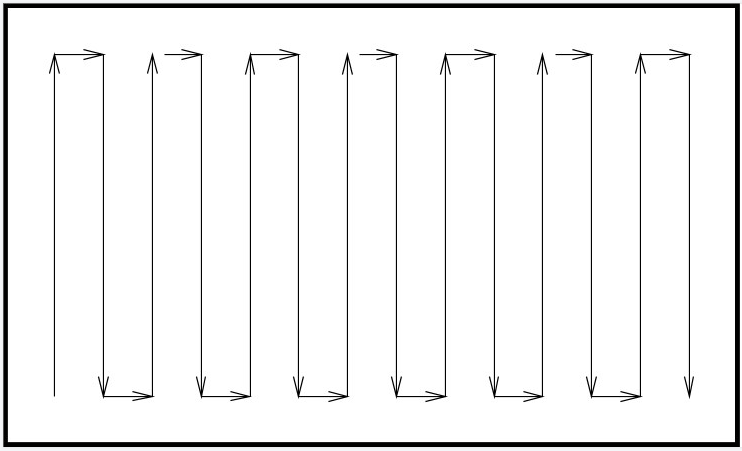
\includegraphics[width=6cm,height=4cm]{RS_Report/bcd.png}
\caption{Diagram of the BCD algorithm\cite{choset1998coverage}. }
\label{bcd}
\end{minipage}
\begin{minipage}[t]{0.48\textwidth}
\centering
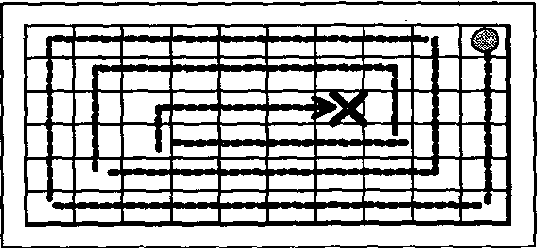
\includegraphics[width=6cm,height=4cm]{RS_Report/BSA.png}
\caption{Diagram of the BSA algorithm\cite{Gonzlez2003BSAAC}.}
\label{bsa}
\end{minipage}
\end{figure}

There is a clear difference between the two algorithms. The BCD algorithm has a tighter overall path because of its 180° turns, which are closer together after each turn, In the BSA algorithm, because of its 90° turns after encountering an obstacle, which is not close together after the turn. BSA algorithm is an outward-to-inward spiral path planning method, and its external route will create a certain distance from the internal route. Its route continuity caused by turning when random obstacles appear in the environment will be relatively poor compared to the BCD algorithm.
Based on these observations, a hypothesis has been developed stating:
\begin{quote}
    In a blank map, the efficiency of BCD and BSA are similar, because both can complete area coverage through a single path planning. However, in a complex map environment (including random obstacles), BCD will be more efficient than BSA. Because BCD has a more compact path than BSA, it reduces the length of the path that the A* algorithm needs to plan between connecting sub-regions.
\end{quote}

\section{Implementation}

\subsection{Overview}

As Fig.\ref{fig3} instructed, The system will obtain the map and the pose of the robot after the program is executed. The map and the pose will be updated at a frequency of 31.25 Hz until the end of the program. Then CCP algorithm will plan the path of a sub-region. The robot will continuously check whether the coverage of the sub-region is completed during the process of tracing. If it is not completed, the robot will continue with the current movement. If completed, the A* algorithm will be used to plan the robot's path to the nearest sub-region. Before executing the A* algorithm, the system will also check whether all sub-regions are covered. If not, execute A*. If yes, the 
program ends.

\begin{figure}[htbp]
\setlength{\belowcaptionskip}{-1cm}
\centerline{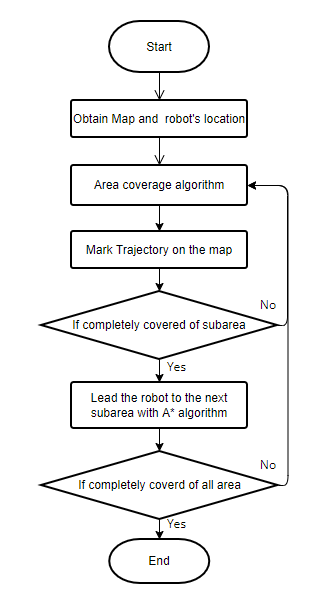
\includegraphics[scale=0.6]{RS_Report/The Overall architecture of the CPP algorithm.png}}
\caption{The flow chart of CPP algorithm.}
\label{fig3}
\end{figure}



\subsection{Map and track tracking system}

The premise of the complete coverage path plan algorithm is a map and locate system. Only when the robot knows the surrounding environment and its position can it make a reasonable path plan.

\subsubsection{Map}

There are various methods to build the environment map, and this experiment mainly uses the raster method\cite{hart1968formal} to build the environment map in a static environment.This method is used because it decomposes the environmental space in to local cells and describes the state of the environment in terms of whether obstacles occupy them or not. The maps produced by this method provide accurate metric information and are easier to understand and process than other methods. Algorithms are compared in 90cm×90cm rectangular maps(see Fig.\ref{fig1}) with obstacles. The robot will receive a static 11×11 raster map (see Fig.\ref{fig2}) at the beginning of the experiment. On the map, cells that contains obstacles or wall are set to 1, and cells that the robot can step on are set to 0.

\begin{figure}[htbp]
\centerline{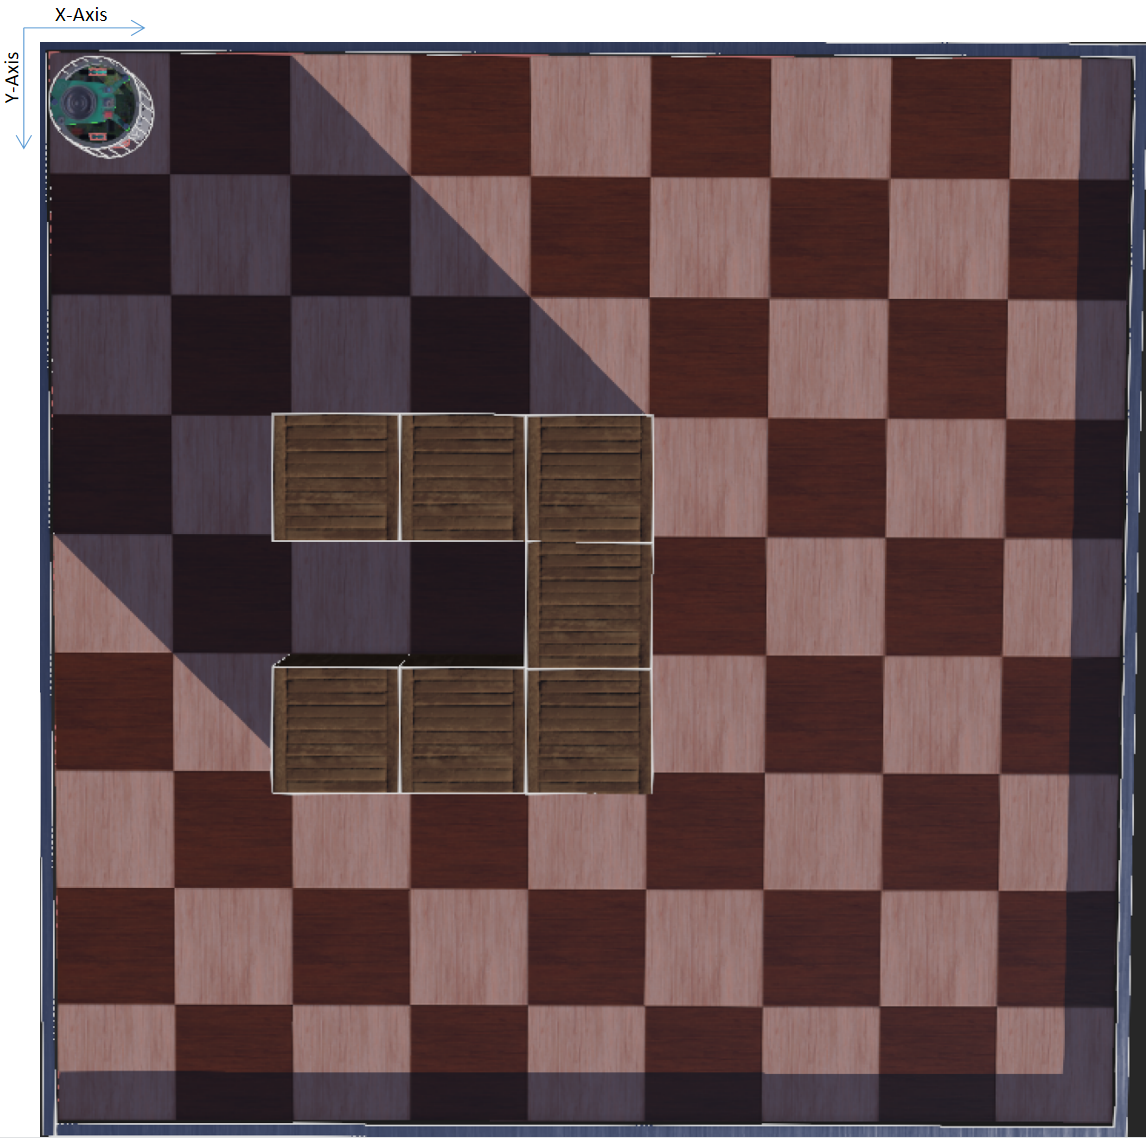
\includegraphics[width=5cm,height=5cm]{RS_Report/Webots_map.png}}
\caption{The experimental map with robot.}
\label{fig1}
\end{figure}

\begin{figure}[htbp]
\setlength{\belowcaptionskip}{-1cm}
\centerline{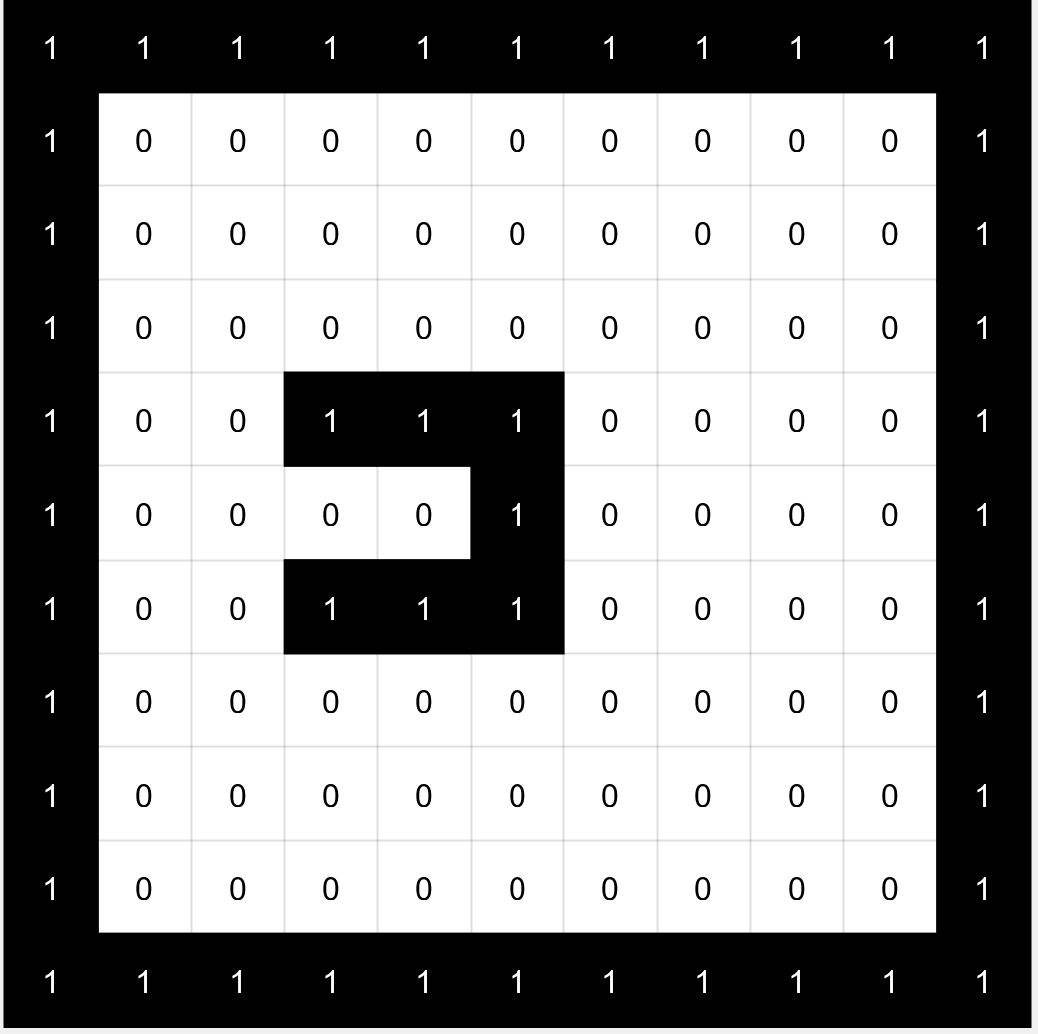
\includegraphics[width=5cm,height=5cm]{map.png}}
\caption{11$\times$11 Raster environment map.}
\label{fig2}
\end{figure}

\subsubsection{robot pose}

In order to obtain the pose of the robot, the supervisor system of Webots is enabled in this experiment. The supervisor system can obtain the absolute position and orientation of the robot in the simulator. The position is information is a three by one translation vector from the simulator's origin to the robot. In this experiment, only x and y are used. The orientation information is returned as Euler angle from the simulator's origin to the robot. Since the robot only walk on the plane perpendicular to the y axis in this experiment, the only useful parameters are the direction of y axis and its angle. The pose of the robot on the map can be obtained by converting the pose obtained from the supervisor. 

\subsubsection{Track tracking}

By storing the pose data of the robot in a list in order, we can get the robot's motion trajectory. In order to more intuitively understand which areas on the map are covered, this trajectory needs to be marked on the map. The 11×11 raster map can only display the position of the robot in integer. Therefore, each punctuation is made when the robot is at the center of the grid. On the raster map, when a cell is covered, the value will change from 0 to 2.

\subsection{CPP algorithm}

\subsubsection{Area coverage path plan algorithm}

The BCD and BSA area coverage algorithms(see Algorithm\ref{alg.l1}) are design with the same finite state machine, but with different motion rules. The robot will behave as the algorithm instructs in different scenarios. The scenarios based on the map and track tracking system updates at a rate of 31.25Hz. The main difference between BCD and BSA lies in the way they turn. The BCD will turn the robot 180 degree in U-shape. The BSA will let the robot implement a 90-degree round turn. That makes the path of the BCD algorithm are lines parallel to each other. The shape of the path of the BSA algorithm is rotated from the outside to the inside. 

\begin{algorithm}[h]
 \caption{Area coverage path plan algorithm}
 \label{alg.l1}
 \begin{algorithmic}[1]
 \Require
 Map; Robot's position on the map;
 \Ensure
 Robot's behavior;
 
    \STATE Wall = 1;
    \STATE Trajectory = 2;
    \STATE Blank = 0;
    \STATE $\textit{Position} \gets \text{Robot's current position on the map}$
    \STATE $\textit{Front} \gets \text{One cell in front of } \textit{Position}$
    \STATE $\textit{Left} \gets \text{The cell to the left of } \textit{Position}$
    \STATE $\textit{Right} \gets \text{The cell to the right of } \textit{Position}$
    {\IF{Front \textgreater 0}
        \IF{Left \textgreater 0}
            {\IF{Right \textgreater 0}
                {The area is fully covered}
            {\ELSE}
                {Turn right}
            \ENDIF
        {\ELSIF{Right \textgreater 0}
            {Turn right}}
        \ENDIF}
  \ENDIF}
  \label{code:recentEnd}
 \end{algorithmic}
\end{algorithm}

Without other path plan algorithms, these two area coverage algorithms can only complete the area coverage of the barrier-free square map. When encountering a complex map with obstacles, they can only cover a part of the map. The area that can be covered by a single path plan is called a sub-regions. For complex maps, to cover the area of the entire map need to divide the map into different sub-regions and cover accordingly. The path from sub-region to sub-region is the plan by the A* algorithm.

\subsubsection{A* algorithm}
The experiment uses the A* algorithm\cite{hart1968formal} to move the robot to the nearest untraversed sub-region until the entire map is traversed. The core of the A* algorithm is
\begin{equation}
  f(n) = g(n) + h(n)
\end{equation}
where $f(n)$ is the combined priority of node n. When the next node to be traversed needs to be selected, the algorithm always picks the node with the highest combined priority (smallest value). $g(n)$ is the cost of node n from the starting point. $h(n)$ is the expected cost of node n from the end point, which is the heuristic function of the A* algorithm.\\
The map entered in Algorithm 1 is redesigned to ensure that the movement of the E-punk on the A* route matches the movement on the area coverage path plan algorithm route. Once the positions of each step in the path have been obtained using the A* algorithm, all positions in this new input map are set to 1, except for the coordinates contained in the A* path, which are set to 0.\\
The traversal direction is simplified in this experiment to match the raster map and speed up the calculation. The mobile robot can only move in four directions, up, down, left and right, in which case the heuristic function is calculated using the Manhattan distance method(see Fig.\ref{fig4}).

\setlength{\belowcaptionskip}{-1cm}
\begin{figure}[htbp]
\centerline{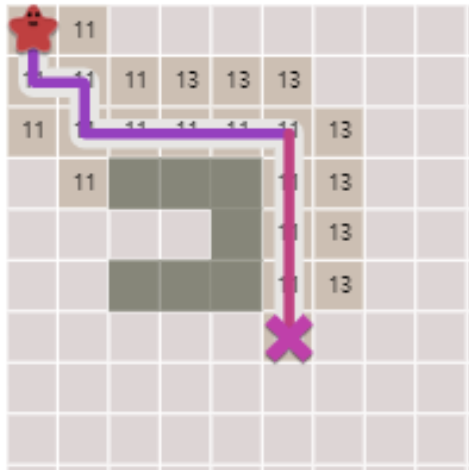
\includegraphics[width=5cm,height=5cm]{RS_Report/astar.png}}
\caption{A* algorithm demonstration(the value in the cell is the value of $f(n)$).}
\label{fig4}
\end{figure}



\section{Experiment Methodology}

\subsection{Overview of Method}
As mentioned in section\ref{Sec1}, the experiments aims to compare the efficiency performance of the two algorithms, BCD and BSA. The simulator used in this experiment is Webots R2021b in Linux. The robot used in the experiment is e-puck robot\cite{Cyberboticswebsite}.\\
The first experiment is carried out in a 60cm$\times$100cm rectangular map without obstacles. Then, the other four experiments are carried out in a 90cm$\times$90cm rectangular map. The size of the obstacle is equal to the size of one cell of the grid map, which is 10cm$\times$10cm. These four maps are designed according to the motion characteristics of the two algorithms. The first map(see in Fig.\ref{fig8.a}) shows the situation where the obstacles are near the center point and symmetrical about the center point. The second map(see in Fig.\ref{fig8.b}) shows the situation where the obstacles is 1-cell offset from the center point. The last two maps(see in Fig.\ref{fig8.c} and Fig.\ref{fig8.d}) shows the situation where obstacles are scattered on the map. The figure of the blank map is not shown because the scene is too simple. The purpose of designing these maps is to compare the efficiency differences of the two algorithms in BSA preferred map and some random map.\\
This paper uses two complete path planning algorithms, BCD and BSA, to experiment on the above-mentioned map. As there is no random error set in the Webots simulator, there is no need to perform multiple experiments in a single map. In order to ensure that there will be no odometry error during the experiment, this paper uses the supervisor system to obtain the robot's pose. 

% Four experimental maps with obstacles
\begin{figure*}[ht]
\centering
\subfigure[ ]{
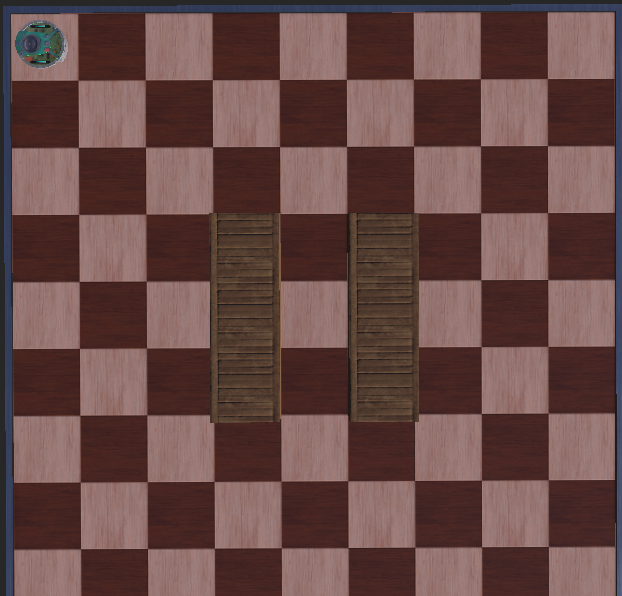
\includegraphics[width=4.3cm,height=4.3cm]{RS_Report/centerial.png}
\label{fig8.a}
%\caption{fig1}
}\hspace{-7mm}
\quad
\subfigure[ ]{
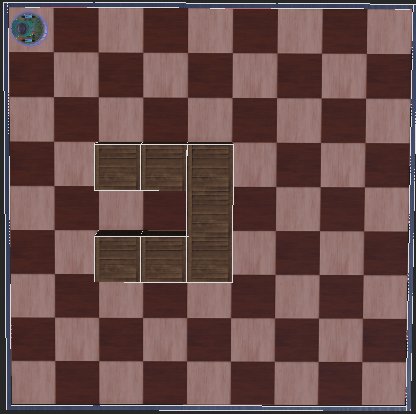
\includegraphics[width=4.3cm,height=4.3cm]{RS_Report/room.png}
\label{fig8.b}
}\hspace{-7mm}
\quad
\subfigure[]{
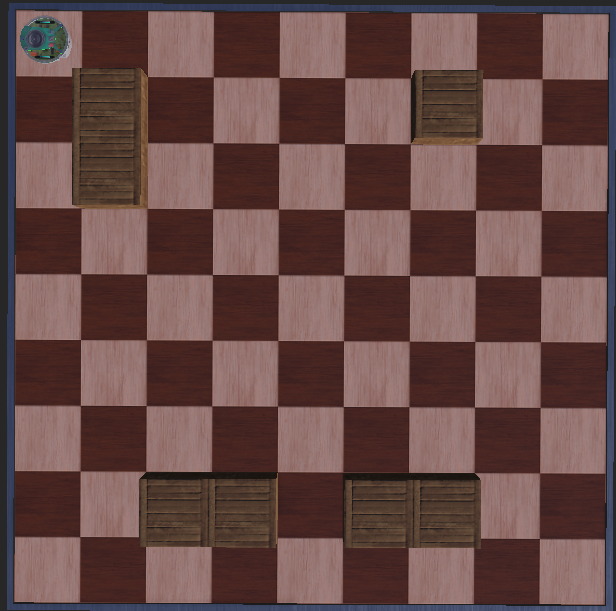
\includegraphics[width=4.3cm,height=4.3cm]{RS_Report/changed_room.png}
\label{fig8.c}
}\hspace{-7mm}
\quad
\subfigure[ ]{
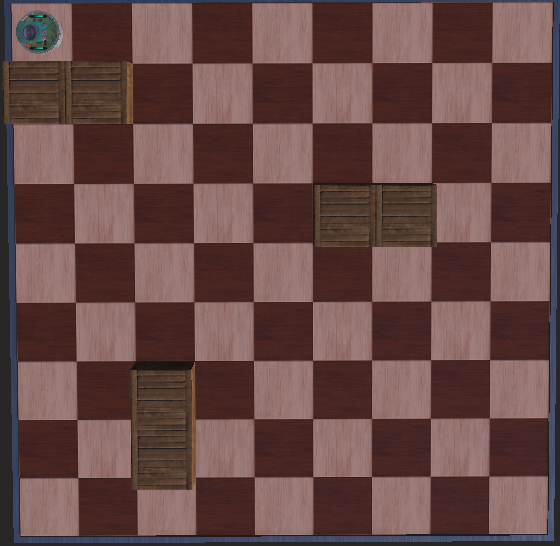
\includegraphics[width=4.3cm,height=4.3cm]{RS_Report/disper_room.png}
\label{fig8.d}
}

\caption{Four experimental maps with obstacles.}
\label{fig8}
\end{figure*}


\subsection{Discussion of Variables}

\subsubsection{Staring point}
In this experiment, it is necessary to control that the initial conditions are the same for both algorithms when comparing on the different complex maps. For the CPP algorithm, it is more efficient to let the robot start from the corner of the map. Therefore, in each experiment, the robot will start from the upper left corner of the view(see in fig.\ref{fig8} and move to the right. The starting position of the robot is set to the point (1, 1) of the map. The orientation of the robot is set to theta equals to zero.

\subsubsection{Velocity}

The maximum forward speed of the e-puck is 0.25 m/s. In the experiments, the speed used by the robot in the experiment is 20$\%$ of the maximum speed, which is 0.05m/s. Both forward and average speed of two wheels when turning are set to be 0.05m/s. The speed is constant for both path planning algorithms, and does not change from one map to another. 

\subsubsection{Turning radius}

For BCD, the radius of the U-shaped bend is set to half the length of the cell, which is 5cm, and the turning angle is 180 degrees. Therefore, the turning path of the robot will cover two cells. For BSA, the radius of the round turn is also 5cm, but the turning angle is 90 degrees. Therefore, the turning path of the robot only covers one cell. 


\subsection{Discussion of Metric(s)}

As proposed in the hypothesis, the metric is for evaluating the two path planning algorithms' efficiency. For the path planning algorithm, the most direct measurement method should be to compare the path length. However, because the two algorithms use the same speed of motion, the length of their path can be indirectly compared by the time for them to complete the task. The time can be obtained by the robot from reading the operation time of the simulator.

Table \uppercase\expandafter{\romannumeral1} Variable summary table.
% The variable summary table
\begin{table}[htbp]
\centering
\setlength{\abovecaptionskip}{0.cm}
\caption{Definition of variable}
\label{Table1}
\begin{tabular}{lll}
\hline
Variables      & BCD               & BSA               \\\hline
Staring point  & upper left corner & upper left corner \\
Forward speed  & 0.05m/s           & 0.05m/s           \\
Turning speed  & 0.05m/s           & 0.05m/s           \\
Turning radius & 5cm               & 5cm               \\
Turning anagle & 180°              & 90°               \\
Metric         & Complete time(s)  & Complete time(s)  \\\hline
\end{tabular}
\end{table}


\section{Results and Analysis}

This experiment compared the BCD and BSA path planning algorithms in a blank map and four complex maps. The time at task completion was obtained using Webots internal timer, which was used to compare the efficiency of the two algorithms. The experimental results are shown in Table \uppercase\expandafter{\romannumeral2}. Fig.\ref{fig7} shows the trajectories of the different path planning algorithms in four complex maps. 

Table \uppercase\expandafter{\romannumeral2} Experimental results table.
% The result table
\begin{table}[htbp]
\centering
\setlength{\abovecaptionskip}{0.cm}
\caption{Presentation of experimental results}
\label{Table1}
\begin{tabular}{lll}
\hline
Maps  & Complete time(s) of BCD & Complete time(s) of BSA \\\hline
Blank & 225.57                  & 225.34                  \\
(a)   & 334.97                  & 299.30                  \\
(b)   & 315.90                  & 326.88                  \\
(c)   & 401.76                  & 412.70                  \\
(d)   & 308.26                  & 370.18                  \\\hline
\end{tabular}
\end{table}


% The Path visualisation diagram for CPP algorith
\begin{figure*}[ht]
\centering
\subfigure[ ]{
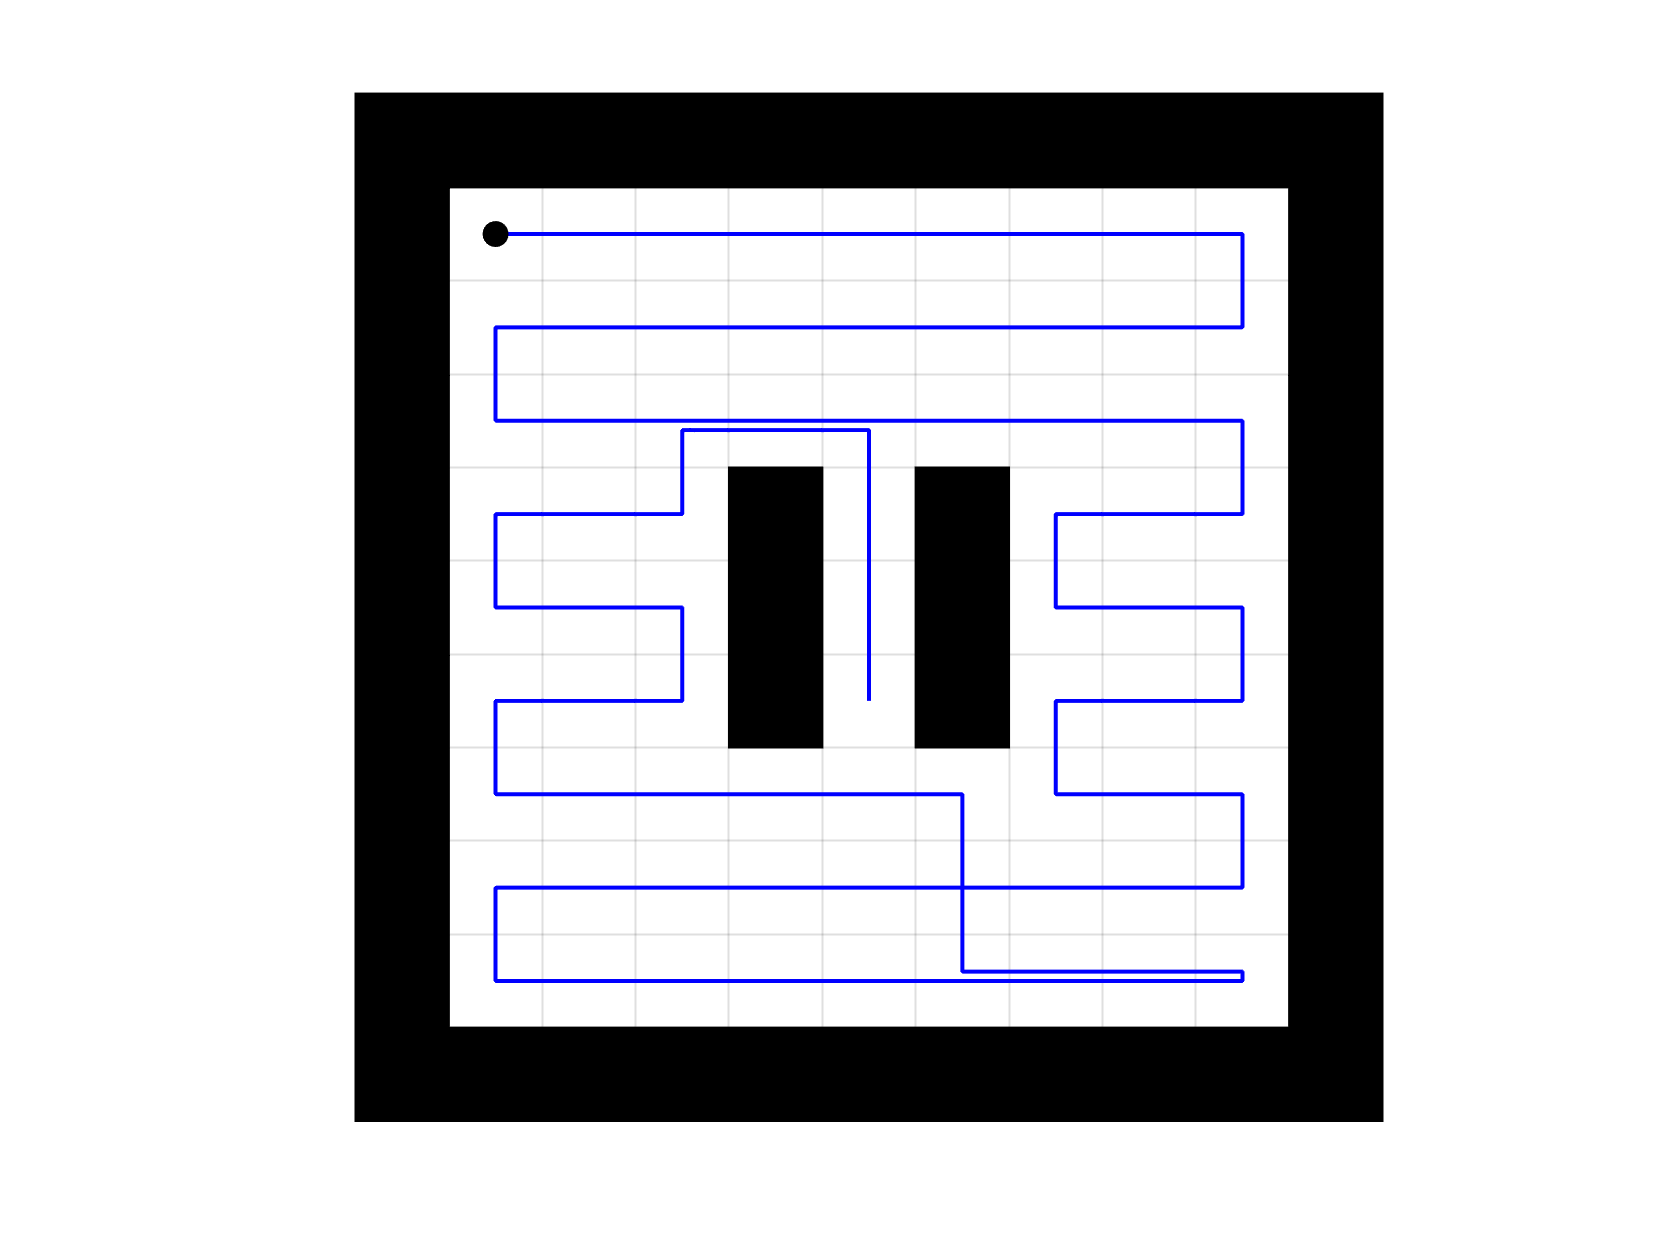
\includegraphics[width=5cm]{RS_Report/BCD_easyMapSS.png}
\label{fig7a}
}\hspace{-16mm}
\quad
\subfigure[ ]{
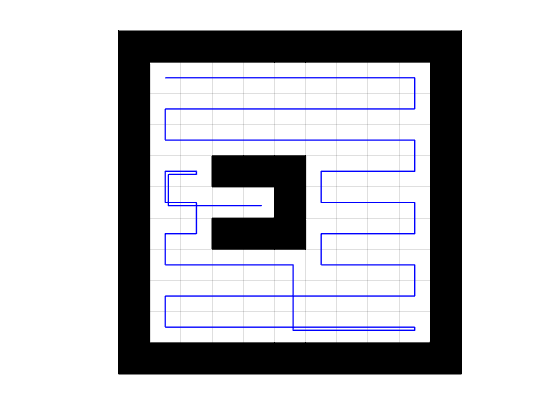
\includegraphics[width=5cm]{RS_Report/BCD_easy.png}
\label{fig7b}
}\hspace{-16mm}
\quad
\subfigure[]{
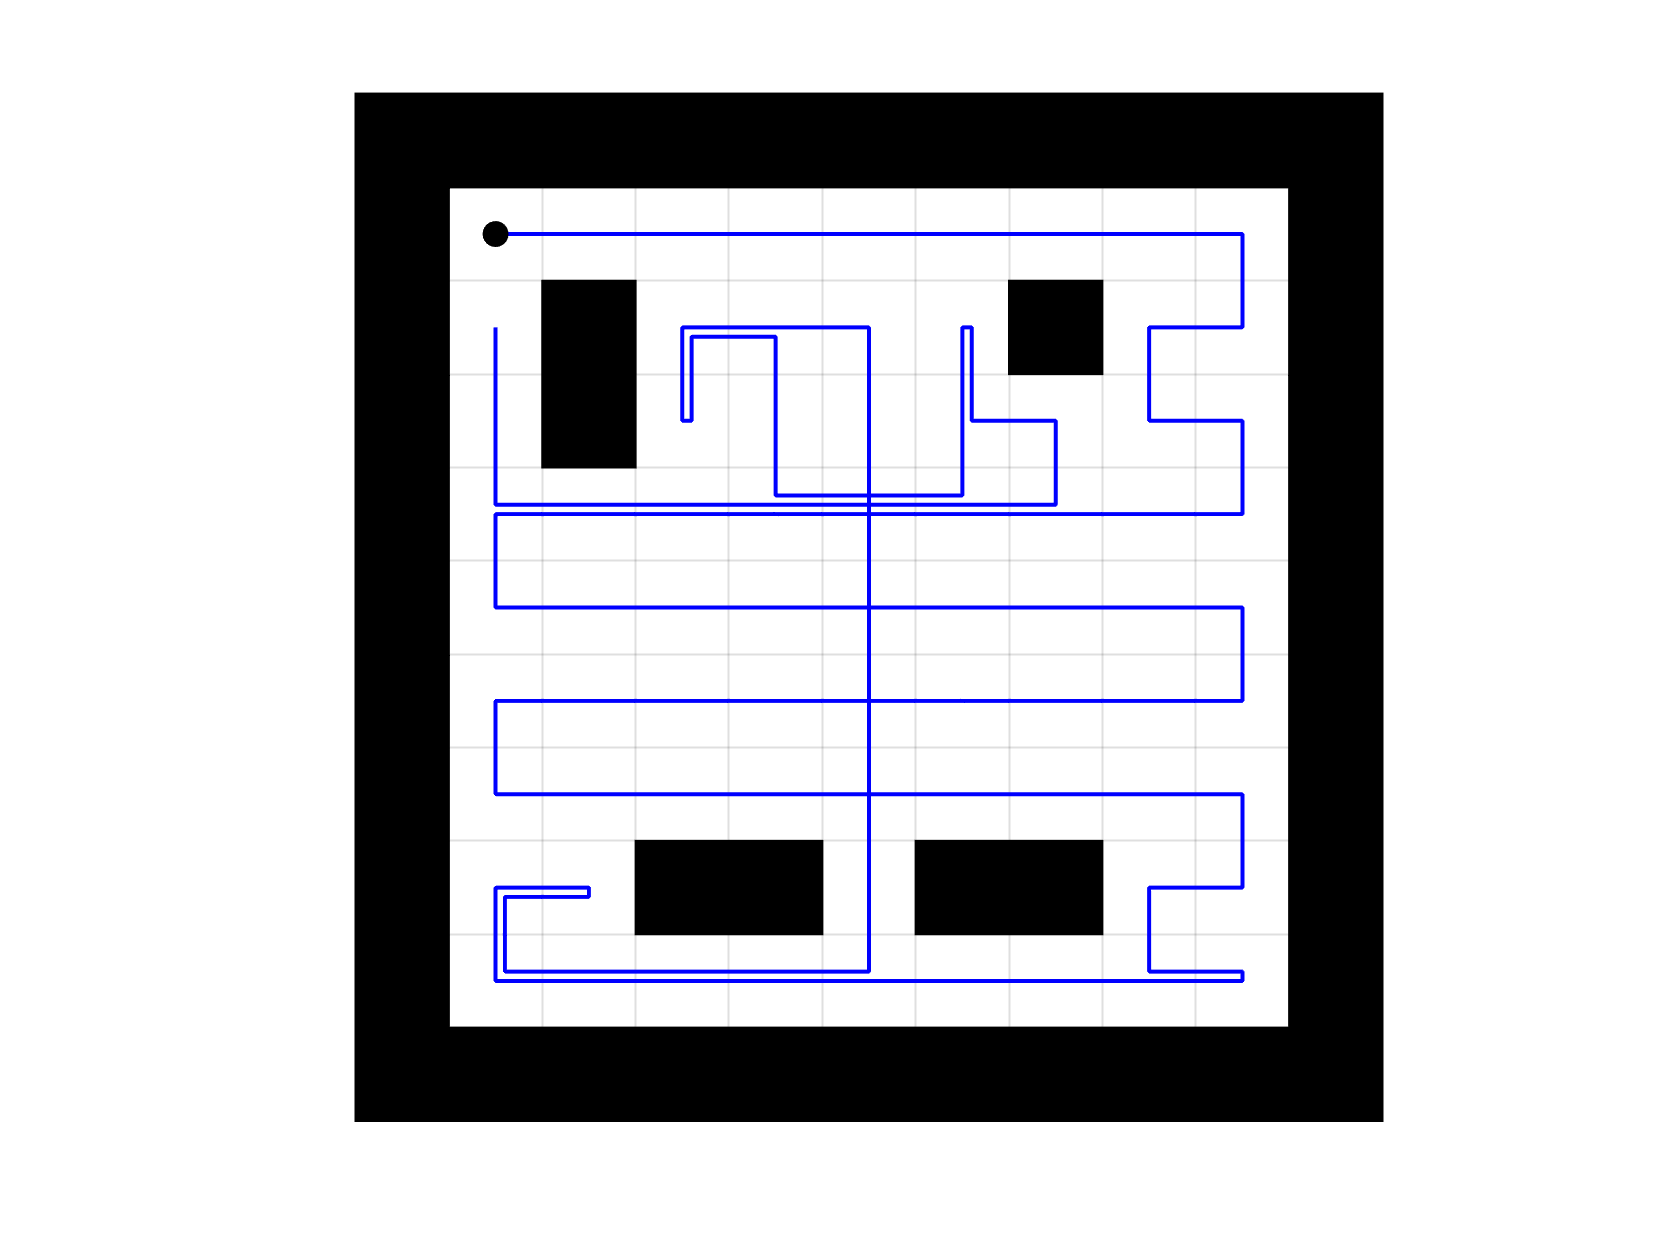
\includegraphics[width=5cm]{RS_Report/BCD_mid.png}
\label{fig7}
}\hspace{-16mm}
\quad
\subfigure[ ]{
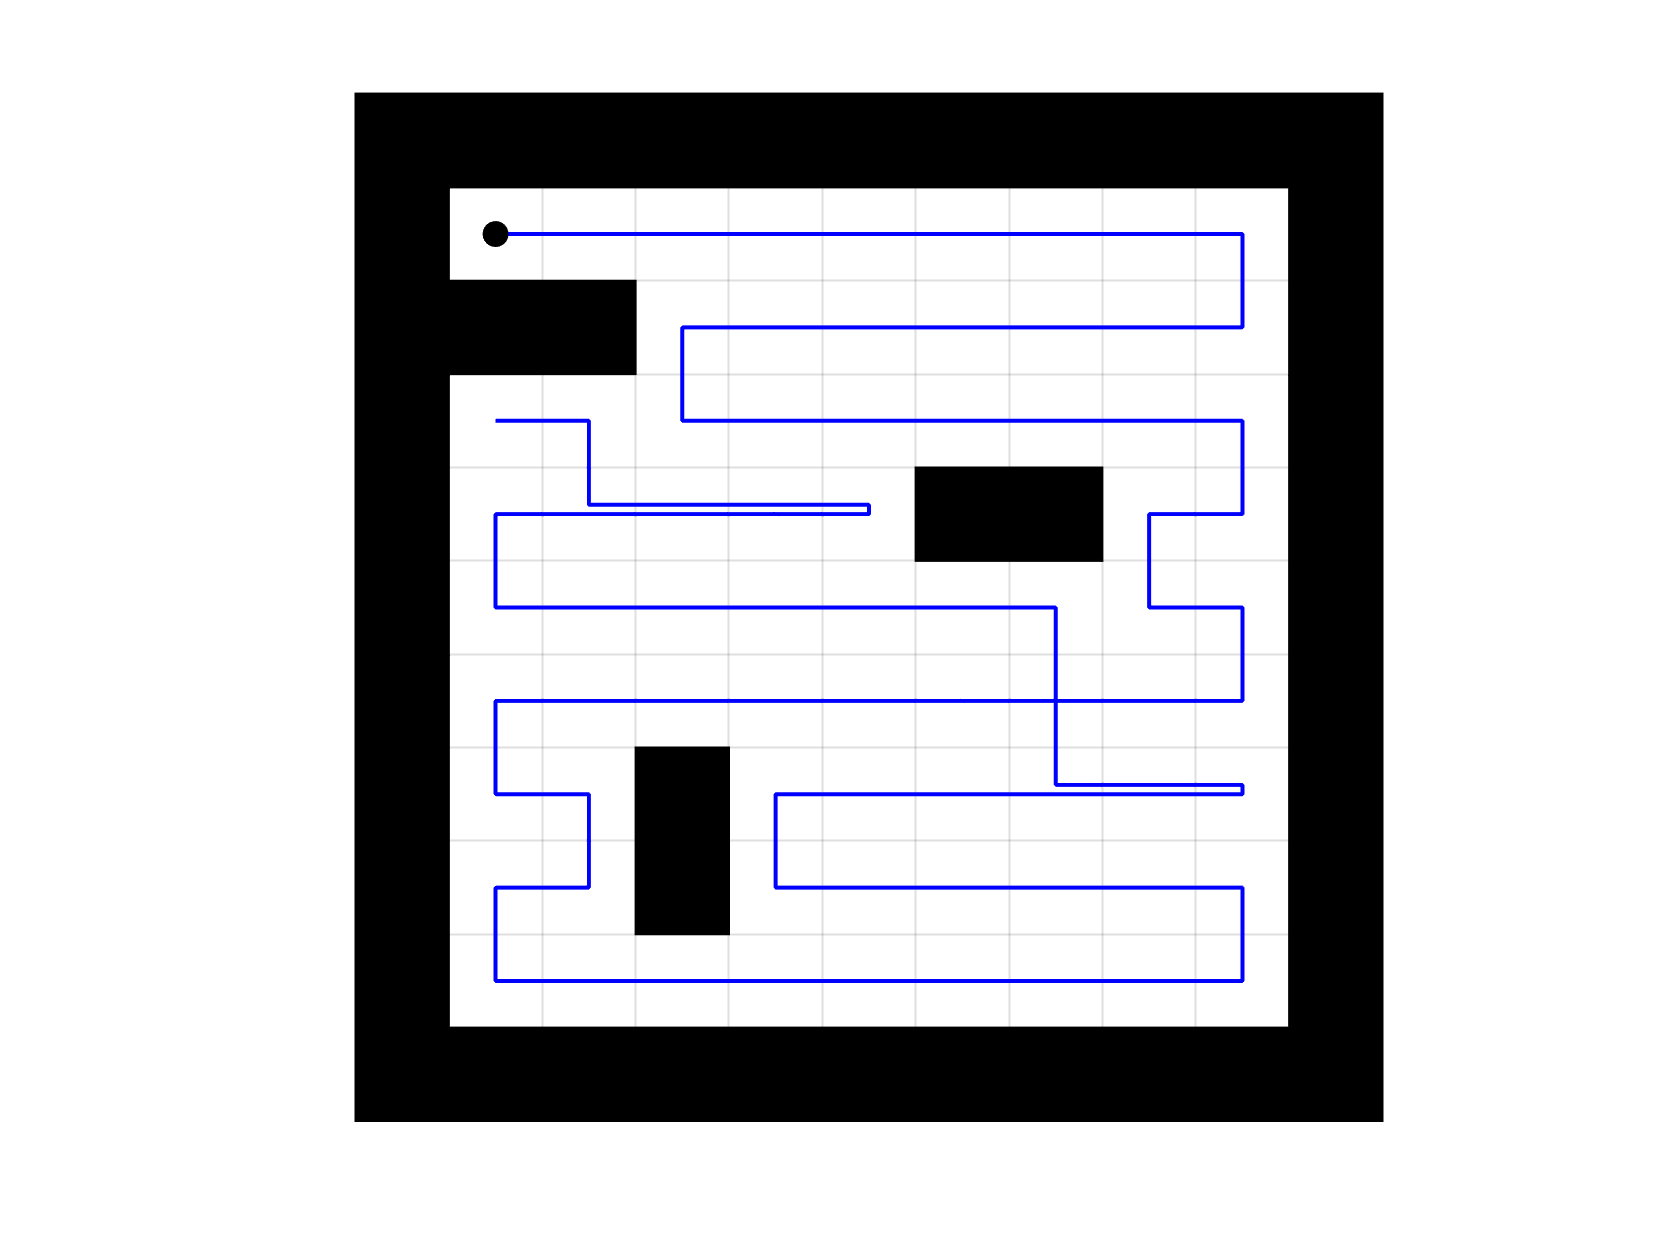
\includegraphics[width=5cm]{RS_Report/BCD_midMapSS.png}}
\label{fig7d}
\quad
\subfigure[ ]{
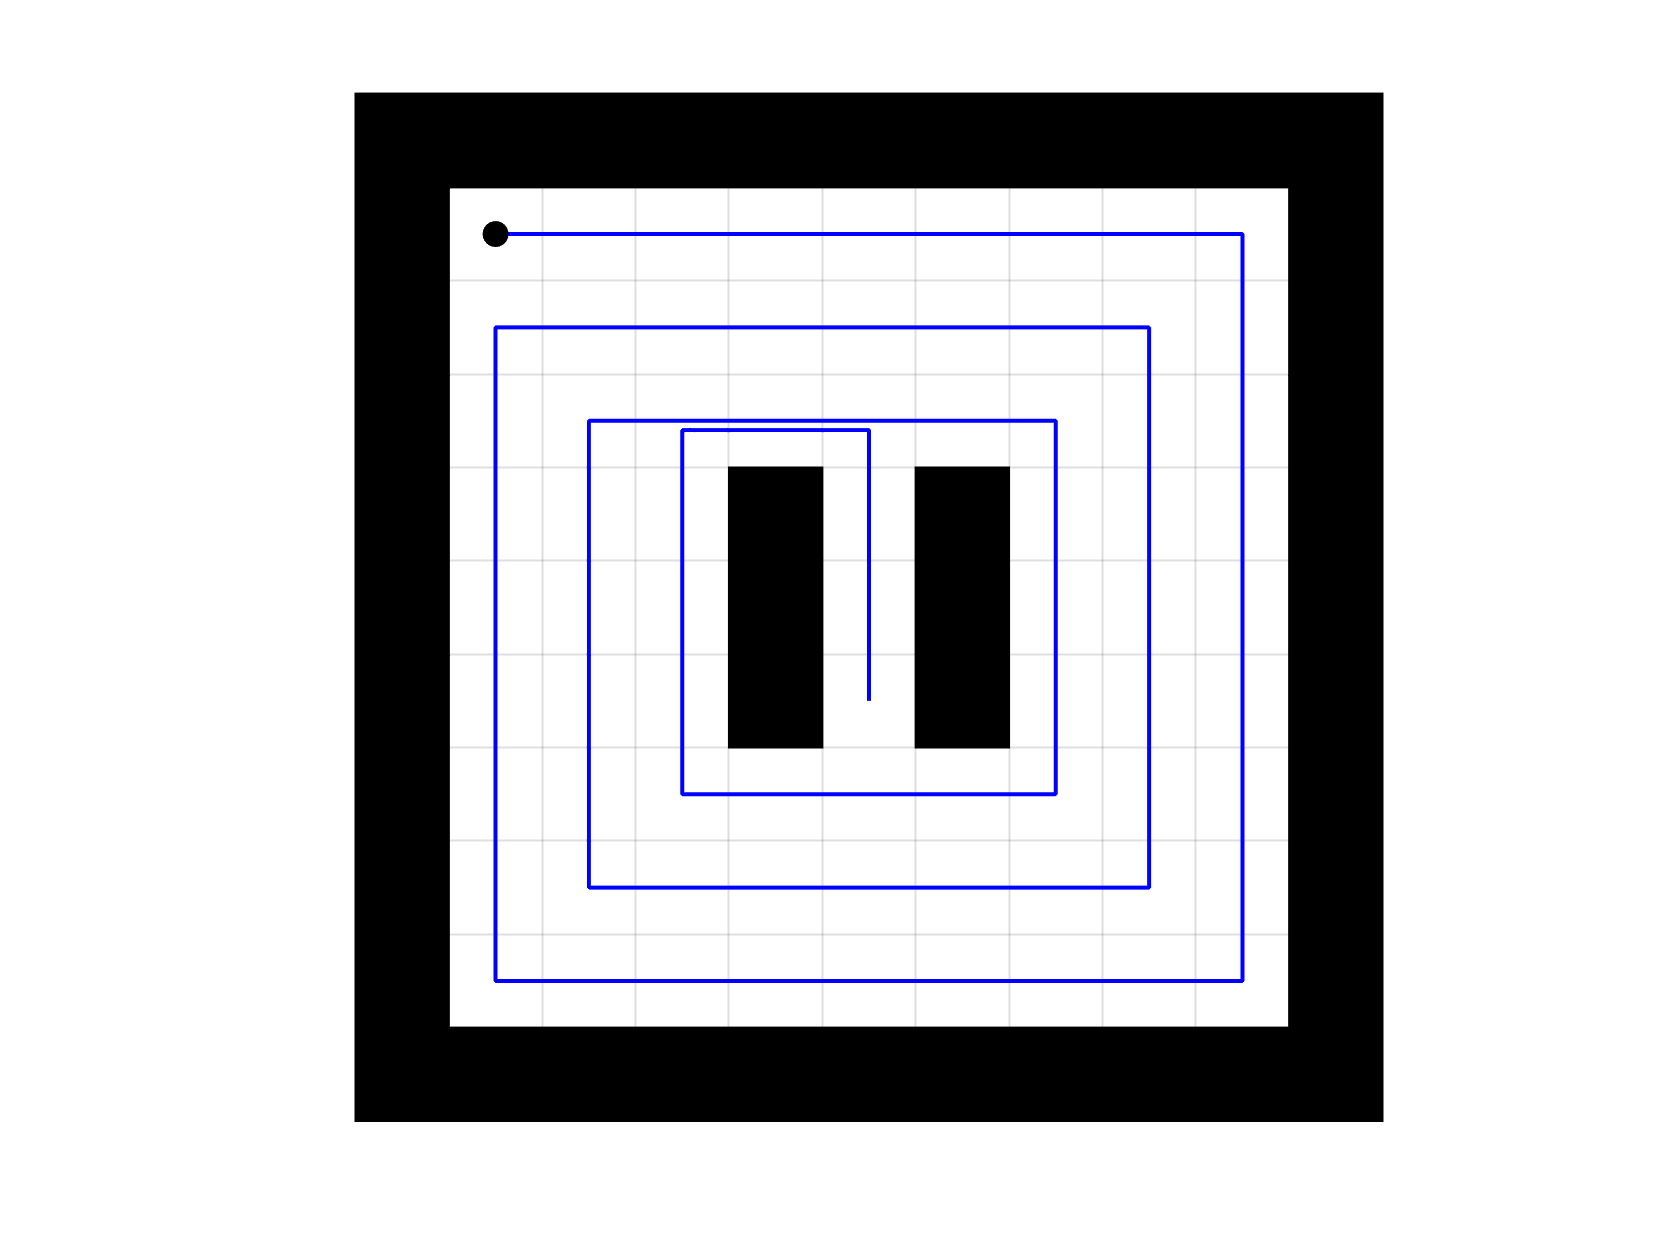
\includegraphics[width=5cm]{RS_Report/BSA_easyMapSS.png}
\label{fig7e}
%\caption{fig1}
}\hspace{-16mm}
\quad
\subfigure[ ]{
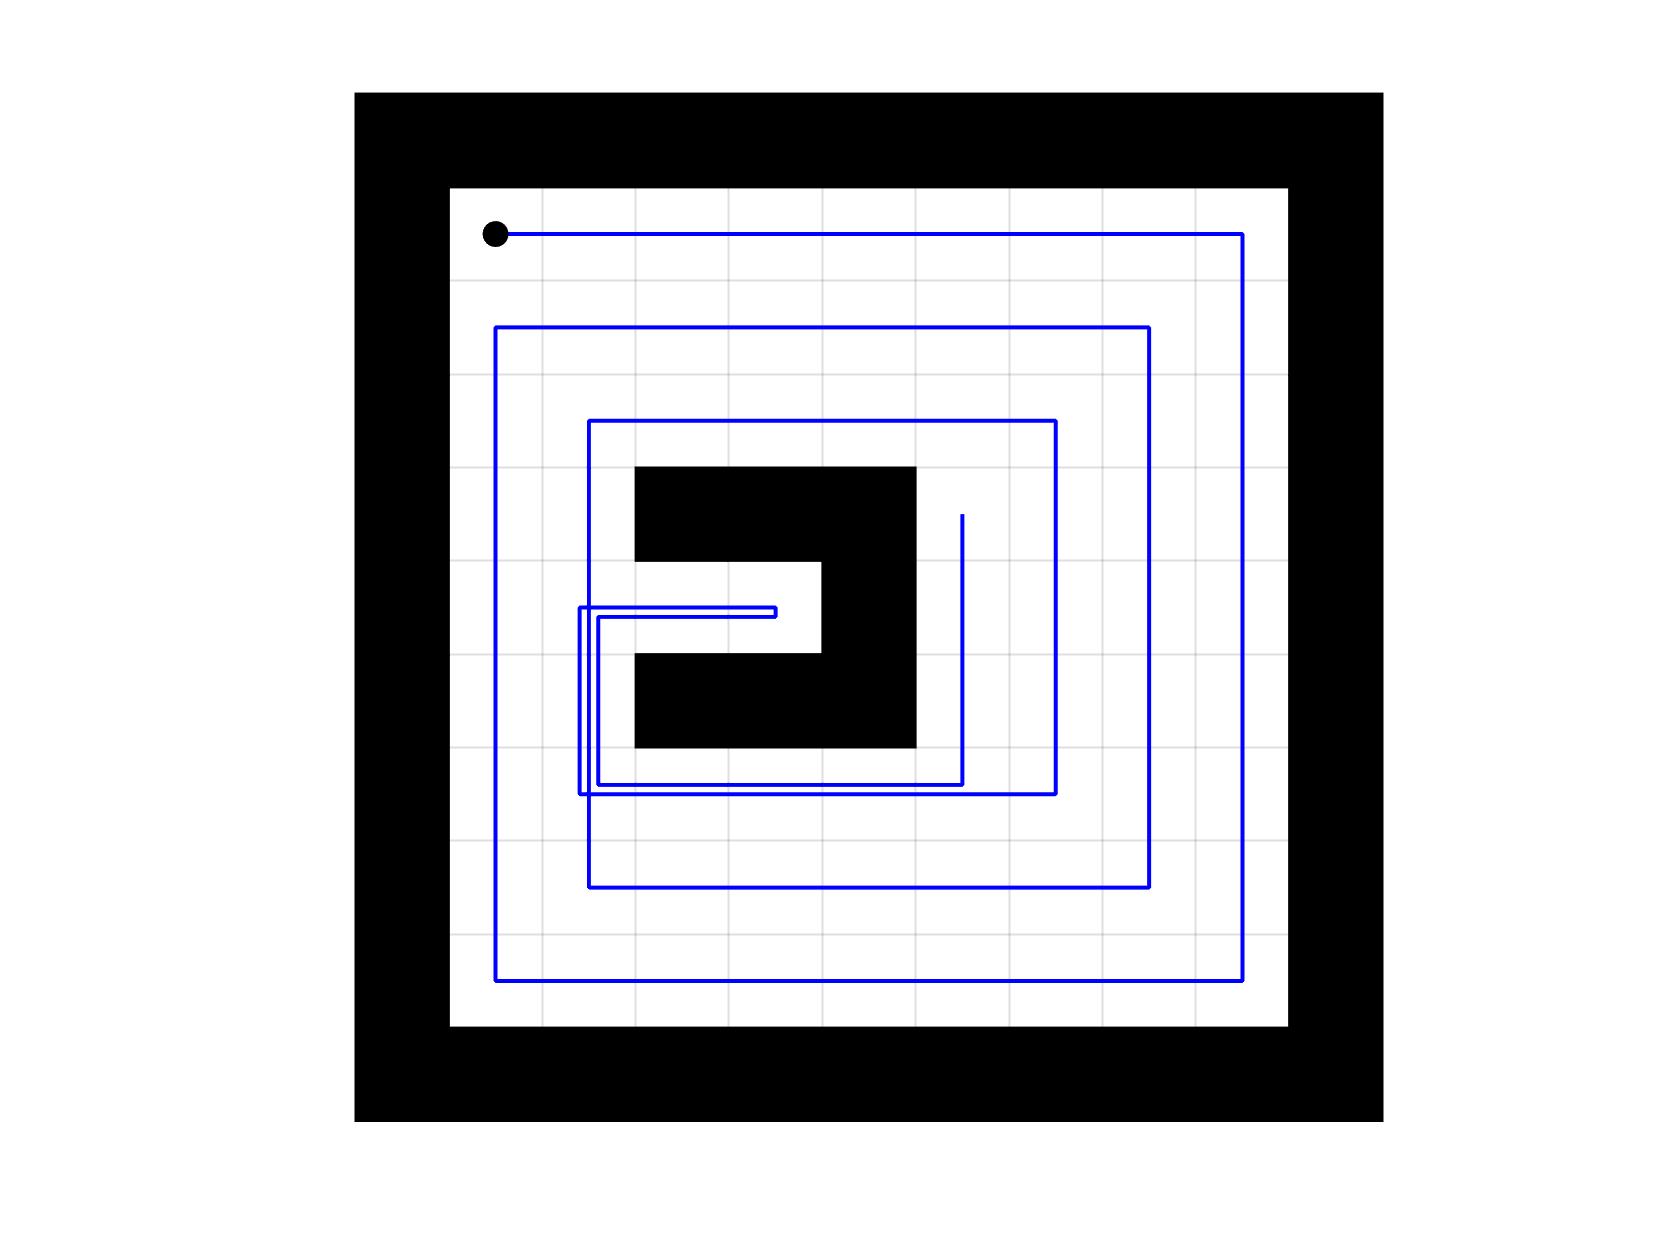
\includegraphics[width=5cm]{RS_Report/BSA_easy.png}
\label{fig7f}
}\hspace{-16mm}
\quad
\subfigure[]{
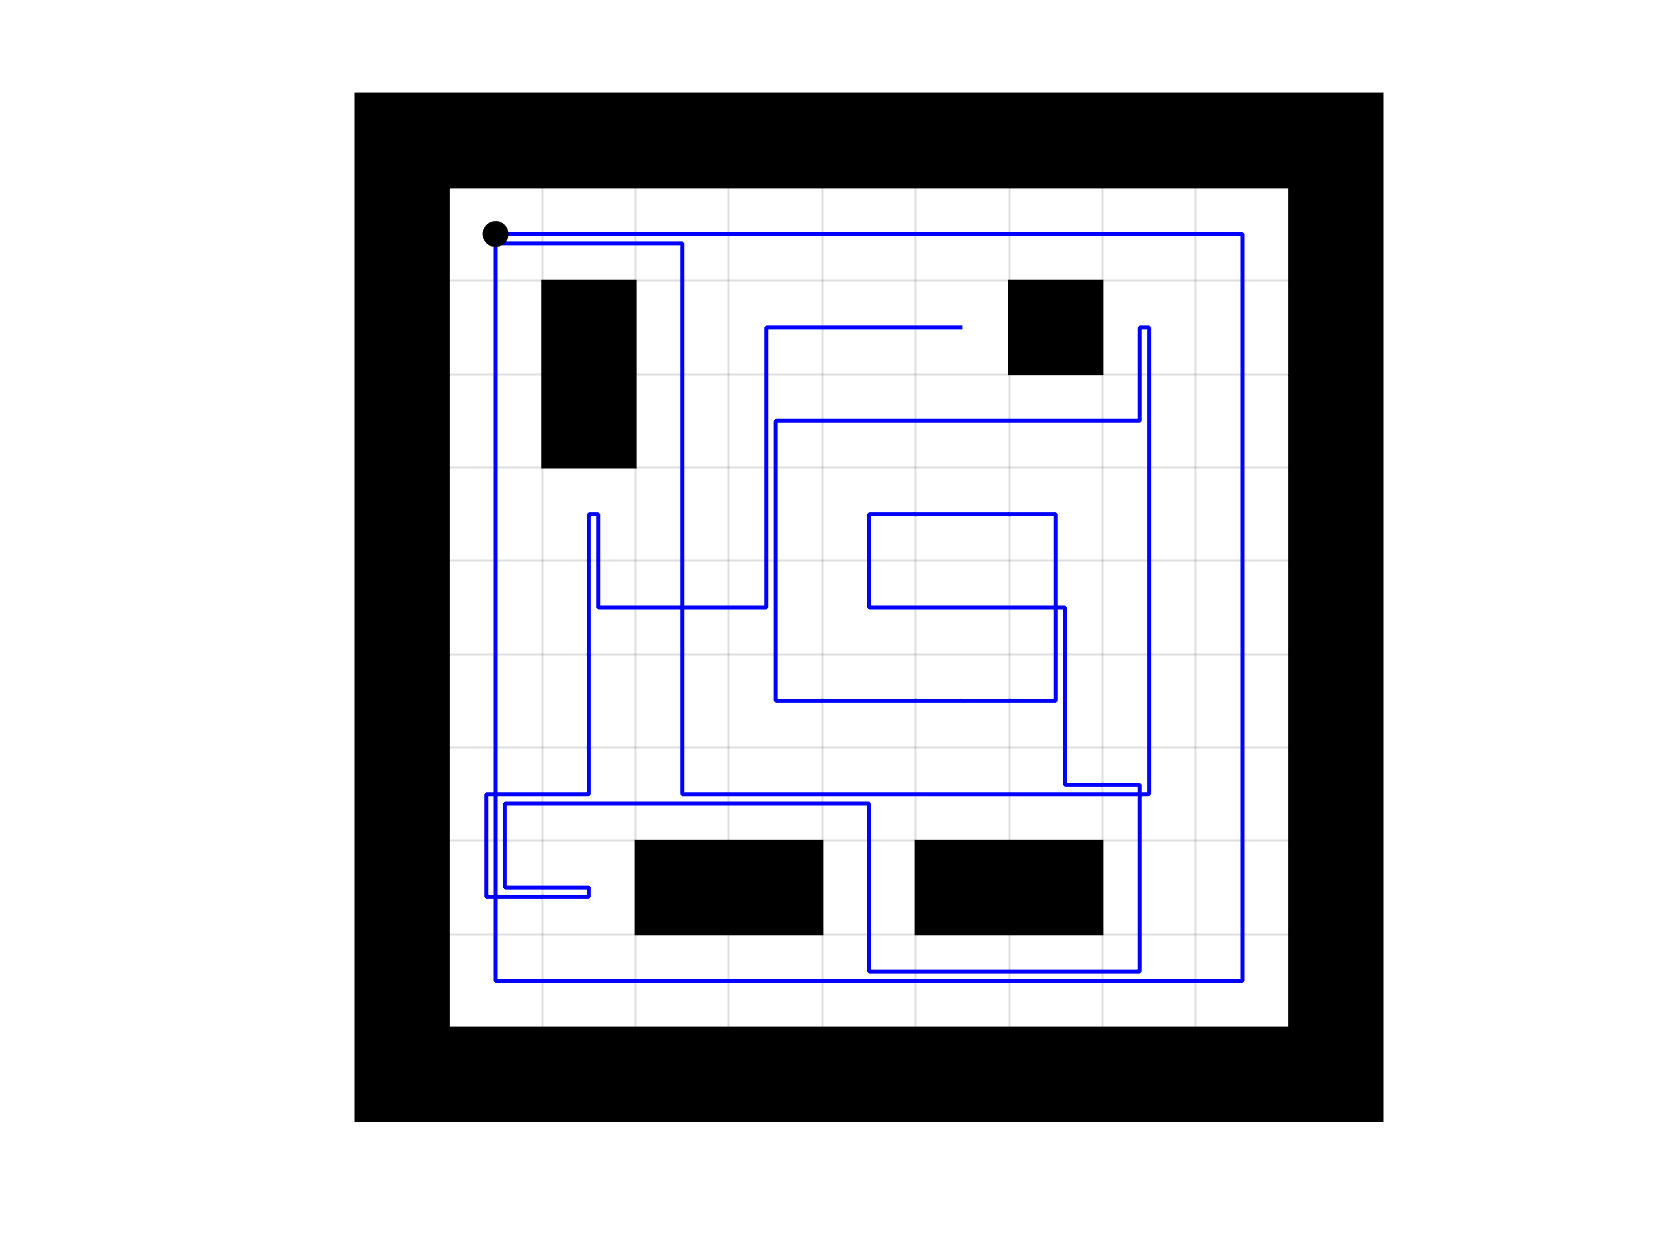
\includegraphics[width=5cm]{RS_Report/BSA_mid.png}
\label{fig7g}
}\hspace{-16mm}
\quad
\subfigure[ ]{
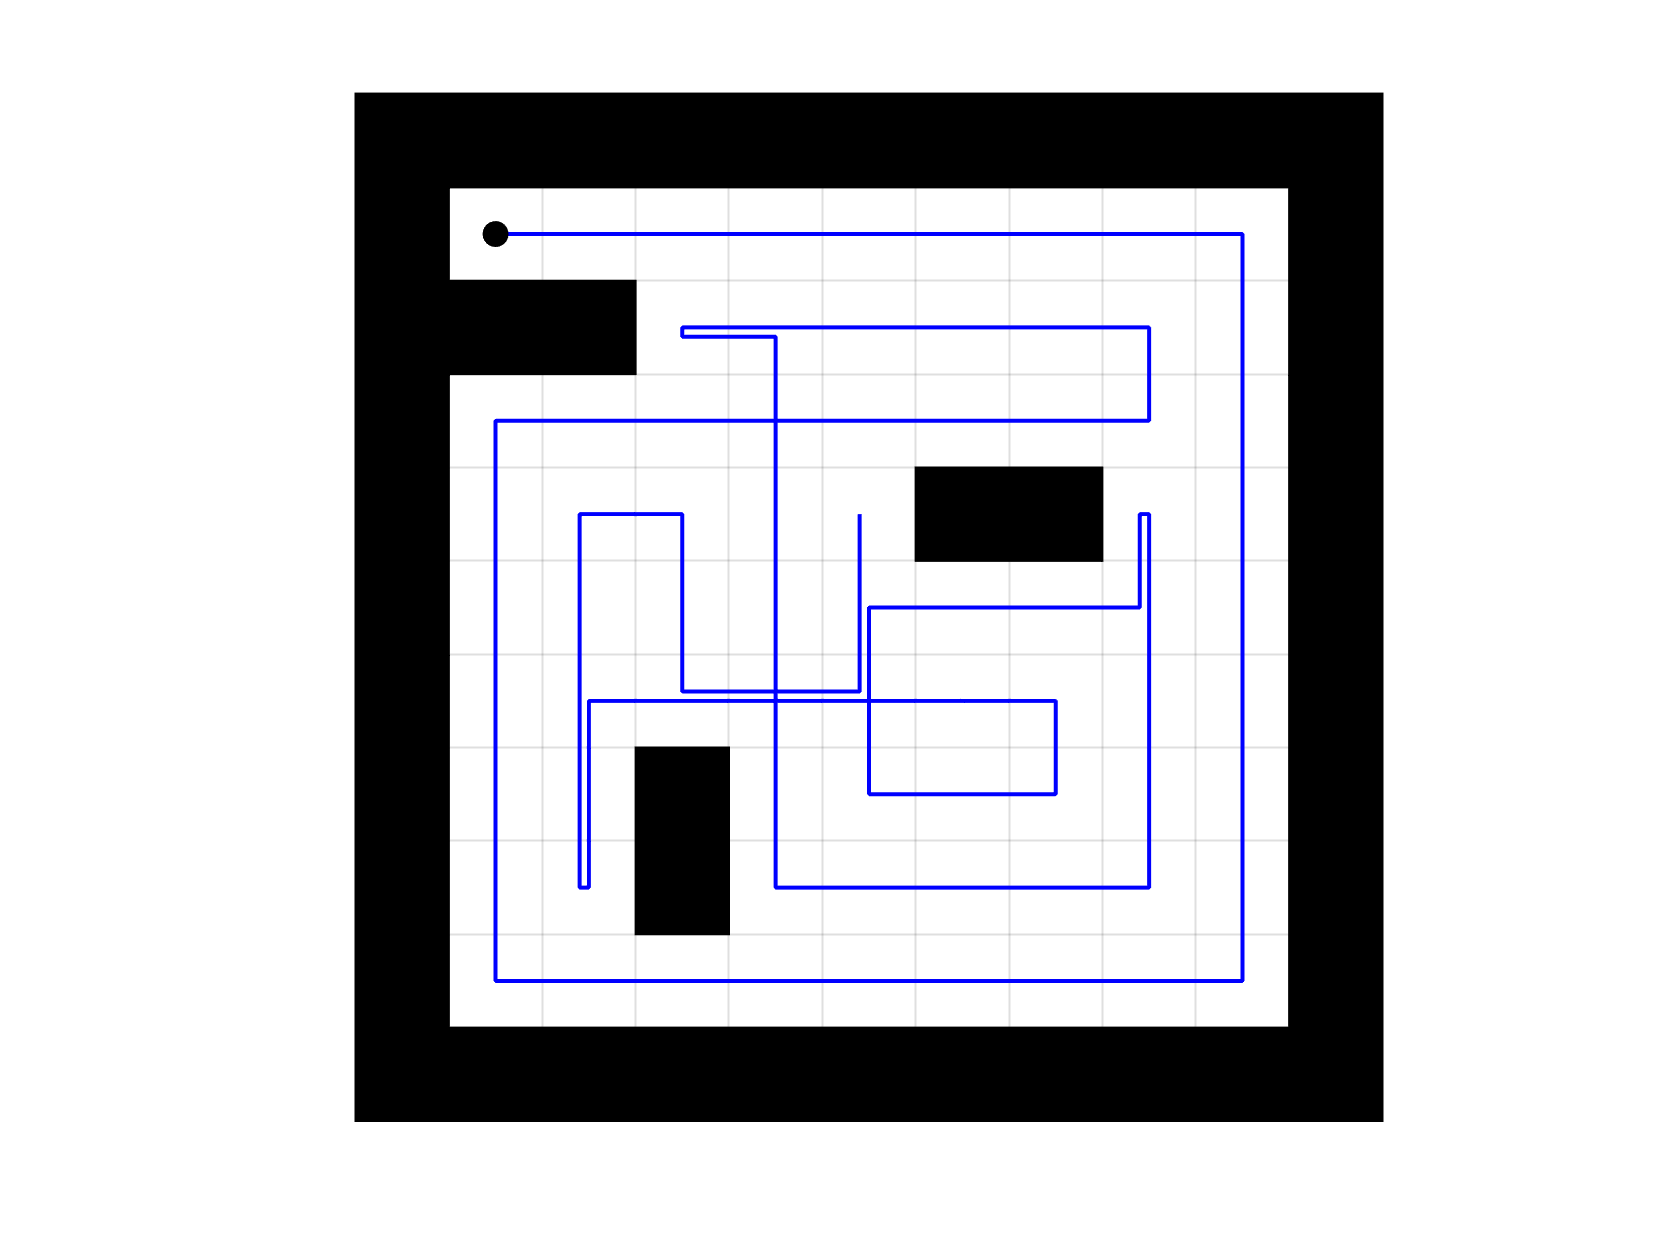
\includegraphics[width=5cm]{RS_Report/BSA_midMapSS.png}
}
\label{fig7h}
\caption{Path visualisation diagram for CPP algorithm.}
\label{fig7}
\end{figure*}


In the blank map, BCD and BSA have similar completion times. The main reason for this result is that there is no significant difference between the lengths travelled by the two algorithms in this map. Furthermore, both algorithms have completed the map traversal without the help of the A* algorithm, therefore there is no repeat path caused by the A* algorithm. Hence, the efficiency of the two algorithms is similar, which also verifies part of the experimental hypothesis.\\
In order to further verify the hypothesis, the author conducted experiments on these two algorithms in four other maps with obstacles.\\
The experimental results show that BSA is more efficient in Fig.\ref{fig8.a}. Because the obstacles in this map are near the center point and are symmetrical about the center point. In this case, most of the BSA path is not affected by obstacles. However, the BCD path will be greatly disturbed by the obstacles, which requires A* algorithm to find the next sub-region for many times. The A* algorithm will guide the robot to take a repetitive path to reached the next sub-region. Therefore, for environments where obstacles near the center point, BSA is a more efficient path planning algorithm.\\
However, in the other three experimental maps, BCD showed higher efficiency. In Fig.\ref{fig8.b} where the  obstacles is 1-cell offset from the center point. Both algorithms use the A* algorithm twice to help complete the map traversal, but it is clear that BSA is not as efficient as BCD because there is a longer A* path in the final path of BSA to complete the traversal. The map partitioning formed by BCD and BSA is different when path planning is completed. Because the route after a BCD turn is adjacent to the one before the turn, the area it passes through is also adjacent and does not result in a repeat of finding points in adjacent areas that have not been traversed. However, BSA does not achieve this effect, resulting in different partitions being far apart, and the efficiency is compromised if there are still obstacles in between.\\
In a map with scattered obstacles like Fig.\ref{fig8.c} and Fig.\ref{fig8.d}, the BCD is still more efficient than the BSA. Especially the results of Fig.\ref{fig8.d}, BCD showed an overwhelming efficiency advantage. The reason for this result is the BSA algorithm suffers from long partition distances. It was also found that when the BSA algorithm encountered an obstacle, the BSA algorithm would miss the points around the obstacle. Therefore, in the area coverage process, the BSA algorithm needs to use the A* algorithm multiple times to reach the points around the obstacle. This process requires repeated traversal of the path, thus affecting efficiency. Compared with BSA, BCD can better cover the cells around obstacles, so it is less dependent on A* algorithm. This is one of the reasons why BCD is more efficient. Fig.\ref{fig7g} and Fig.8(h) show that because BSA is a spiral inward motion mode, this tends to increase the distance of the spiral center from the next point found by the A* algorithm, thereby increasing the amount of time to reach the next position. \\
In summary, as long as the obstacles deviate from the center point, BSA loses its efficiency advantage. BCD will be more efficient than BSA in complex environments. This is also in line with the experimental hypothesis. 

\section{Conclusion and Recommendations for Further Work}

This paper aims to compare the efficiency performance of two different CPP algorithms in different map environments. The experimental result has verified the hypothesis that both algorithms, BCD and BSA, have similar efficiency performance in maps without obstacles. However, in a map containing obstacles, when the obstacles are located near the center point, BSA has higher efficiency. Except for this situation, the results of BCD experiments are better than BSA. Therefore, the hypothesis of the thesis is partially correct.\\
It should be noted that the CPP algorithm contains the A* algorithm. BCD is more efficient than BSA in the experiments because the A* algorithm paths between different regions in BCD are shorter and the A* algorithm paths are tighter to the paths traversed by the map, especially around obstacles compared to the paths in BSA.

Further work could include:
\begin{itemize}
  \item [1)]
    The heuristic function used in the experimental A* algorithm is the Manhattan distance, which is a method that allows movement in only four directions in the raster map: up, down, left and right. This A* algorithm does not provide an optimal solution for the shortest path between two points, and this method is not the most efficient one. Further work could improve the heuristic function by using the diagonal distance as the heuristic function if the e-puck is allowed to move diagonally towards the neighbouring node. If the e-puck can move in any direction within the map, the Euclidean distance can be used as a heuristic function.
  \item [2)]
    The CPP algorithm used in the experiment did not calculate the optimal path. Because the calculation of the optimal path requires geometric division of the map, which requires the use of more complex image processing algorithms. Optimal partitioning of the map can greatly reduce the length of paths that need to be traversed repeatedly, thereby improving efficiency.
  \item [3)]
    In this experiment, the maps used in the experiment are all 9$\times$9 raster maps. The efficiency of the two algorithms in larger scenarios needs further testing. In addition, only the case where the obstacle is rectangular was tested in the experiment. For more complex shapes, such as circular or irregular obstacles, requires future tests. Compared with the complex and dynamic real-world working environment of vacuum robots, the test environment of this experiment needs to be improved.
    
\end{itemize}



\bibliographystyle{ieeetr} 
\bibliography{biblio}


\end{document}
